\section{Endelige metode}
\subsection{Metoderne}
\subsubsection{Sparse Label Dictionaries}	% Marcus
%\textbf{Disclaimer der måske skal med: SLD er en metode udviklet af Anders noget fra DTU, vi har set metoden til et foredrag men har ikke set noget litteratur der beskriver metoden udførligt. Dette er derfor vores udlægning af SLD-metoden}\\
%\\
%SLD er en metode til at klassificere forskellige elementer i et givent billede. I SLD vælger man et passende udsnit af kandidatbilledet hvorefter 


%Sparse Label Dictionaries-metoden (SLD) vælger man et passende udsnit af kandidatbilledet således at udsnittet kommer til at indeholde de forskellige klasser af elementer man ønsker at dedektere samt

Sparse Label Dictionaries metoden (SLD) har til formål at segmentere billeder. SLD opretholder to matricer med information om image patches, den ene indeholder intensiteten og den anden den assosierede label information.

SLD opbygger disse to matricer i to trin, første trin er at initialisere matricen. Dette gøres ved at se på to billeder, et træningsbillede samt et billede hvor ground truth er markeret. Fra starten vælges så en størrelse på det udsnit man ønsker at arbejde med. En atom klippes så ud af træningsbilledet i pixel (0,0) og med størrelse $\sqrt{n}\times\sqrt{n}\times h$, hvor $n$ er antallet af pixels i udsnittet og h er farvedybten, så f.eks. 1 ved grayscale og 3 ved RGB billeder. Denne atom gemmes så i intensitetsmatricen. I præcis samme område klippes en atom ud af ground truth billedet der så gemmes i labelmatricen. En skematisk illustration af denne proces ses i figur \ref{fig:postmethod_intensitydict_init} og \ref{fig:postmethod_labeldict_init}. Ground truth billedet har også h dimensioner, hvor hvert segment der ønskes at detekteres er markeret men en farve. Vores udsnit flyttes så en pixel, hvorefter det samme gøres igen. Det vil sige at hvis træningsbilledet er $m\times m$ og vores atom størrelse er $n\times n$ så samler vi $(m-n+1)^2$ billeder. 

\begin{figure}[H]
		\centering
		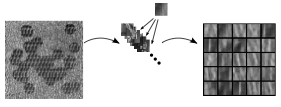
\includegraphics[scale=1]{files/postmethod/img/dict_1.png}
	\caption{Billedudsnit ekstraheret fra træningsbilledet og lagt over i intensitetsmatricen. \label{fig:postmethod_intensitydict_init}}
\end{figure}

\begin{figure}[H]
		\centering
		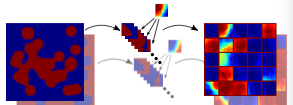
\includegraphics[scale=1]{files/postmethod/img/dict_2.png}
	\caption{Det tilsvarende ground truth billede med associerede udsnit ekstraheret og lagt i labelmatricen.\label{fig:postmethod_labeldict_init}}
\end{figure}

For at bygge de mest optimale billeder, ønsker vi at labelmatricen indeholder unikke billeder for hver klasse. Dette gøres ved at der vælges et tilfældigt subset af udsnittene fra træningsbilledet, og ved en iterativ proces, undersøges det hvorvidt det associerede labelatom allerede er tilnærmelsesvis repræsenteret i labelmatricen, og tilføjes kun hvis det ikke er tilfældet. Dette sikrer både at størrelsen på matricerne bliver minimeret der gør at listen er hurtigere at gennemgå, samt at billedudsnit med lignende intensiteter og labels tilhører samme matriceatomer. 

Når matricerne er fyldt op med intensitet- og labelatomer begynder en ny algoritme at optimere på matricernes indhold. Ideelt set vil en pixel i en labelatom have sandsynligheden 1 for en klasse og 0 for alle andre klasser. Algoritmen forsøger at opnå dette ved iterativt at opdele atomerne i klasser og redigere i label sandsynlighederne. 

Med de færdigbyggede matricer kan SLD gå igang med at segmentere billeder. Metoden starter typisk med at modtage et testbillede der bare kan være testbilledet med akserne ombyttet. Denne proces er dog kun for at teste at de matricer man har opbygget rent faktisk kan segmentere de klasser man ønsker.

\begin{figure}[H]
		\centering
		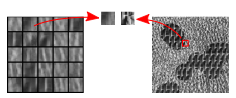
\includegraphics[scale=1]{files/postmethod/img/dict_3.png}
	\caption{\label{fig:postmethod_sld_imagepatch}}
\end{figure}

Processen med at segmentere et billede med de to matricer starter ligesom når matricerne blev opbygget. Udsnit størrelsen på $\sqrt{n}\times\sqrt{n}$ vælges, hvor $n$ igen er antallet af pixels i udsnittet, og løber igennem det billedet der ønskes segmenteret på samme vis som da vi fyldte matricerne. For hvert udsnit findes den atom, $d^*$, i intensitetsmatricen som Euklidisk ligger tættest på billedudsnittet ved ligningen
\begin{align}
	d^* = min_j ||d_j-x||
\end{align}

Dette er skematisk illustreret i figur \ref{fig:postmethod_sld_imagepatch}, hvor firkanten til højre repræsenterer det billede der ønskes segmenteret, og firkanten til venstre repræsenterer intensitetsmatricen. 

Herefter hentes den tilsvarende label ud fra labelmatricen og tilføjes til det nye segmenterede billede. Hver atom man tilføjer til det nye billede adderes oveni de allerede indsatte pixels hvilket betyder at hver pixel i det resulterende billede består af bidrag fra $n$ labelatom pixels, og som er et gennemsnit af sandsynlighederne af alle labels der dækker denne pixel. Denne labeling proces ses illustreret i figur \ref{fig:postmethod_sld_labelpatch}. Bemærk at siden dette er en binær segmentering, så har labelatomet to label dimensioner.  

Labelbilledet med den højeste intensitet bestemmer så det resulterende binære billede. Et eksempel på dette, hvor labelprocessen er halvejs ses i figur \ref{fig:postmethod_sld_resulting}.

\begin{figure}[H]
		\centering
		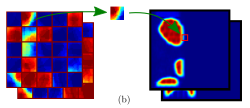
\includegraphics[scale=1]{files/postmethod/img/dict_4.png}
	\caption{\label{fig:postmethod_sld_labelpatch}}
\end{figure}

\begin{figure}[H]
		\centering
		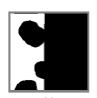
\includegraphics[scale=1]{files/postmethod/img/dict_5.png}
	\caption{\label{fig:postmethod_sld_resulting}}
\end{figure}

Skaberne af SLD beskriver metoden som værende en forbedring i forhold til andre lignende metoder, da den kun indeholder en matrice af intensitetsatomer selvom der er flere klasser. Samtidig er metoden stærk selv overfor billeder med meget støj og træningsbilleder med labels i dårlig kvalitet. I figur \ref{fig:postmethod_sld_testing} vises i første linje tre testbilleder med hhv. 5, 16, 10 og 2 klasser der skal segmenteres. I anden linje ses ground truth af disse billeder. I tredie linje ses resultatet efter segmenteringen. Her ses det tydeligt at hver klasse er segmenteret og der kun er segmenteringsfejl i overgangen mellem klasserne. Billederne er bl.a. behandlet med et gaussisk filter med standard afvigelse på 1.5 og udsnitstørrelse på $3\times3$.

\begin{figure}[H]
		\centering
		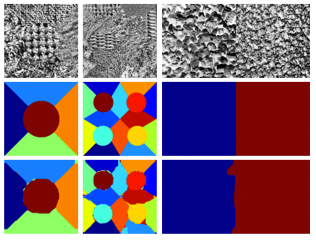
\includegraphics[scale=1]{files/postmethod/img/dict_6.png}
	\caption{Testbilleder øverst, ground truth i midten og resultatet af segmenteringen nederst.\label{fig:postmethod_sld_testing}}
\end{figure}

\subsubsection{Vores implementation af SLD}

\subsubsection{Foldning med eksempelbilleder}
Som vi har nævnt i tidligere afsnit, har vi opnået de bedste resultater efter at lede efter vesiklerne selv, i stedet for at lede efter egenskaber som kanter og andet. Vi forsøger derfor så at detektere vesiklerne ved at folde med billeder af disse. Vi laver derfor en liste af vesikler der hver repræsenterer en type vesikel. Da der er forskel på vesiklernes farve, form og størrelse er det nødvendigt men denne liste af vesikler, i stedet for bare at nøjes med en enkelt. Vi tager så hver enkelt vesikel og folder med billedet. Et eksempel på et område vi ønsker at finde vesikler i, og den vesikel vi folder med, ses i figur \ref{fig:postmethod_conv_pre}.

\begin{figure}[H]
	\begin{minipage}[b]{0.5\linewidth}
		\centering
		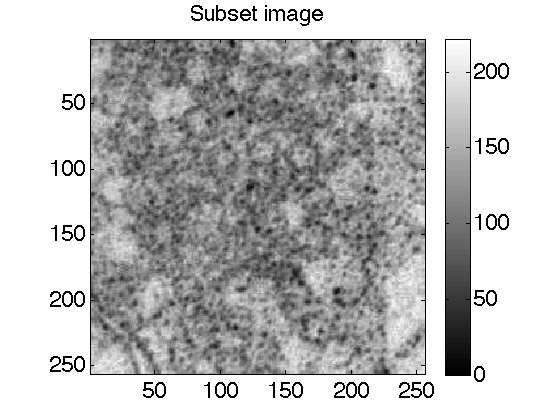
\includegraphics[scale=0.5]{files/postmethod/img/conv_1.png}
	\end{minipage}
	\hspace{0.5cm}
	\begin{minipage}[b]{0.5\linewidth}
		\centering
		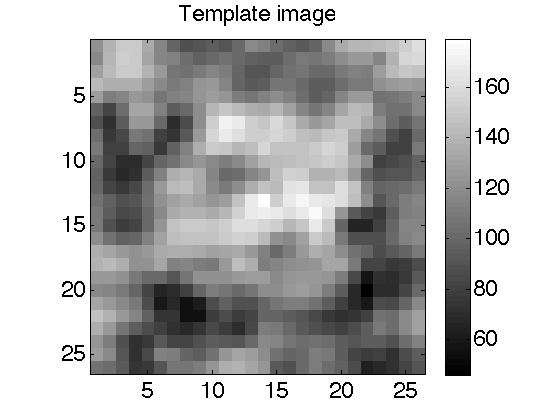
\includegraphics[scale=0.5]{files/postmethod/img/conv_2.png}
	\end{minipage}
	\caption{Til venstre ses en celle hvor vi ønsker at detektere vesikler. Til højre ses den vesikel der ledes efter.\label{fig:postmethod_conv_pre}}
\end{figure}

Udregningen af værdierne i hver pixel gøres med ligningen

\begin{align}
	\sum \left(\frac{I_{udsnit}-mean(I_{udsnit})}{std(I_{udsnit})}-\frac{J-mean(J)}{std(J)}\right)^2 \label{ali:postmethod_conv}
\end{align}
hvor $I_{udsnit}$ er et udsnit af det originale billede I på størrelse med $J$, hvor $J$ er vesiklen. Funktionen tager altså et område på samme størrelse som den eftersøgte vesikel, normerer hver indgang i dem begge for at de er på samme skala, trækker dem fra hinanden og kvadrerer resultatet. Summen af dette er så den Euklidiske afstand mellem de to områder.

Rent teknisk fungerer dette ligesom SLD metoden tidligere beskrevet. Vi tager et udsnit, her et billede af en vesikel, og placerer i pixel (0,0). Summen ovenfor udregnes så for området og gemmes i centerpixlen, altså her i (0,0). Hvis udsnittene vi vælger går ud over kanten af billedet indsættes 0'er i de manglende felter. Vi flytter så området en enkelt pixel og gør det samme igen. Modsat SLD udregner vi altså her kun en værdi for hver pixel. 

Det resulterende billede indeholder så fra 0 og opefter. Hvis et udsnit ligner den vesikel der søges efter, vil $I_{udsnit}$ og $J$ i (\ref{ali:postmethod_conv}) jo være næsten ens, sumfunktionen vil altså gå imod 0 alt efter hvor godt området ligner. Omvendt vil sumfunktionen give høje værdier hvis området ikke ligner den eftersøgte vesikel. Da høje værdier er lig med hvid, og værdier mod 0 er lig med sort, vil det resulterende billede altså have mørke områder hvor der er fundet vesikler. Et eksempel på et sådant billede ses til venstre i figur \ref{fig:postmethod_conv_post}. Til højre i samme figur ses det samme billede, hvor de mørkeste pixelværdier er markeret med hvidt i det sorte canvas.

\begin{figure}[H]
	\begin{minipage}[b]{0.5\linewidth}
		\centering
		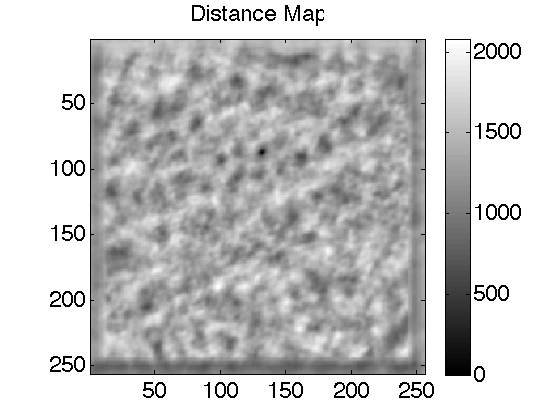
\includegraphics[scale=0.5]{files/postmethod/img/conv_3.png}
	\end{minipage}
	\hspace{0.5cm}
	\begin{minipage}[b]{0.5\linewidth}
		\centering
		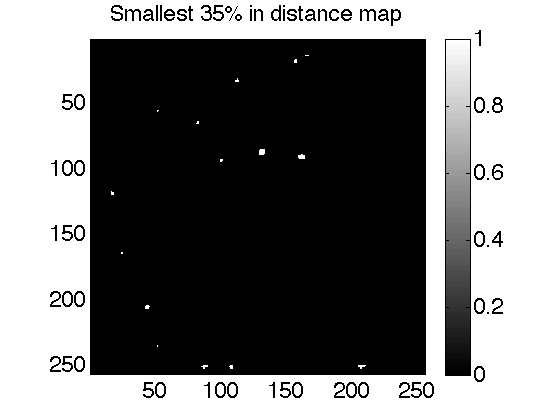
\includegraphics[scale=0.5]{files/postmethod/img/conv_4.png}
	\end{minipage}
	\caption{Til venstre ses en celle hvor vi ønsker at detektere vesikler. Til højre ses den vesikel der ledes efter.\label{fig:postmethod_conv_post}}
\end{figure}

For lettere at se markeringen af vesiklerne har vi plottet de fundne områder med farver i det originale billede på figur \ref{fig:postmethod_conv_photoshop}. De grønne områder er de vesikler som funktionen korrekt har markeret, altså sande positive. De blå områder er hvor funktionen ikke har markeret nogen vesikler selvom de i virkeligheden er der, altså falske negative. Til sidst er der områderne markeret med rødt. Dette er områder som funktionen har markeret som vesikler selvom der ikke er nogen, altså falske positive. Dette betyder altså at ground truth i billedet er de grønne samt i blå.

I eksemplet her er der altså fundet 7 sande positive, 6 falske negative og 8 falske positive. Dette giver en sensitivity (sand-positiv-ratio) på
\begin{align}
	SPR = \frac{SP}{SP+FN} = \frac{7}{13} = 0.538
\end{align}
og antallet af fejldetekterede vesikler (fejl-ratio) er
\begin{align}
	FR = \frac{FP}{FP+SP} = \frac{8}{15} = 0.533
\end{align}

\begin{figure}[H]
		\centering
		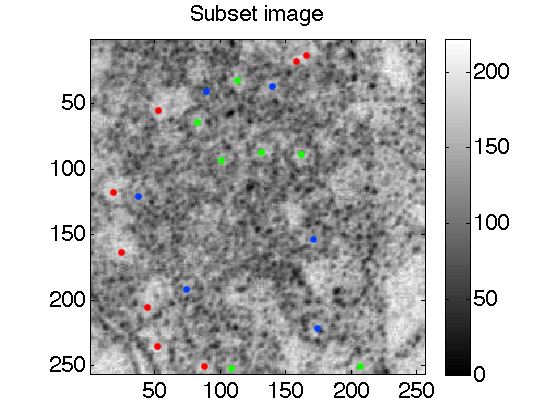
\includegraphics[scale=1]{files/postmethod/img/conv_5.png}
	\caption{Oprindelige billede med markerede områder. Grønne er korrekt detekterede vesikler. Røde er forkerte detekterede vesikler. Blå er vesikler det ikke blev detekteret.\label{fig:postmethod_conv_photoshop}}
\end{figure}

Som det ses på billedet er der både flere falske positive og falske negative. Resultatet er dog efter en foldning med en enkelt vesikel. Vi kan derfor vælge at regulere tærskelværdien for hvor tæt de fundne områder skal være på 0. At hæve tærskelværdien kan medføre at vi finder flere vesikler, men også flere falske positive, hvorimod at sænke tærskelværdien kan reducere antallet af falske positive, men kan dog også fjerne et antal af de sande positive. I forhold til vores igangværende eksempel kan vi prøve at se på hvordan tærskelværdien ligger. Ser vi f.eks. på området omkring den korrekt fundne vesikel i nedre højre hjørne, kan vi plotte værdierne omkring denne. Dette har vi gjort i figur \ref{fig:postmethod_conv_lines_1}, hvor vi også har tegnet en linje ud fra 700 på y-aksen, da dette er vores nuværende tærskelværdi. Vi ved fra ground truth at der i dette område ikke er flere vesikler, hvorfor at vi kan se at vi ikke skal hæve tærskelværdien til mere end ca. 780 før at der vælges flere falske positive. 

\begin{figure}[H]
		\centering
		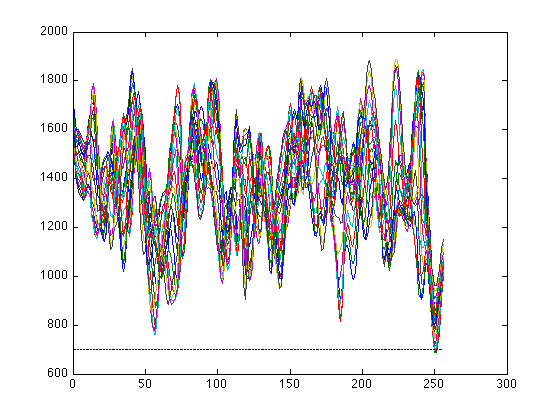
\includegraphics[scale=0.9]{files/postmethod/img/conv_lines_1.png}
	\caption{Udregnede værdier i området fra 200 til 220 på x-aksen. \label{fig:postmethod_conv_lines_1}}
\end{figure}

Omvendt har vi i figur \ref{fig:postmethod_conv_lines_2} plottet området omkring to falske positive vesikler. Her kan vi aflæse at vi ved at sænke tærskelværdien til f.eks. 600 ville slippe af med disse. Går vi så tilbage og ser på figur \ref{fig:postmethod_conv_lines_1} ser vi dog at dette vil medføre at den korrekt detekterede vesikel ikke vil blive detekteret.

\begin{figure}[H]
		\centering
		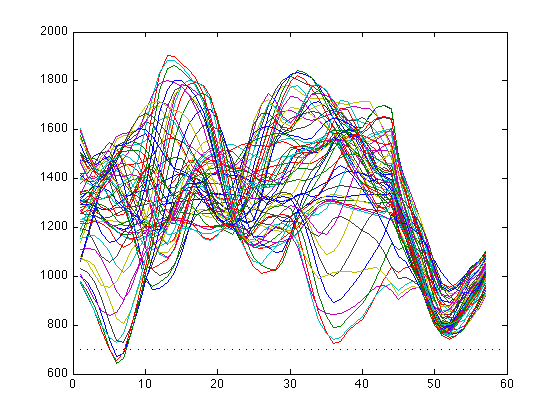
\includegraphics[scale=0.9]{files/postmethod/img/conv_lines_2.png}
	\caption{Udregnede værdier i området fra 1 til 60 på x-aksen, og 200 til 255 på y-aksen. \label{fig:postmethod_conv_lines_2}}
\end{figure}

Da vores algoritme folder med en liste af vesikler er vi dog mere interesserede i at den finder færre vesikler, mod at den holder antallet af falske positive nede. Vores mål er da at tage de fundne vesikler efter hver foldning, og kombinere til et endeligt resultat. I nedenstående tabel ses vores resultater efter forsøg med forskellige tærskelværdier og forskellige  vesikler. Alle vesiklerne er fra billedet som der efterfølgende foldes med. Vi viser kun de resultater der har fundet andre vesikler end den der foldes med. I SPR og FR søjlerne har vi markeret de bedste værdier for hver vesikel.

\begin{figure}[H]
	\centering
\begin{tabular}{l|l|l|l|l|l|l|l}
	$\#$ & Vesikel & Tærskelværdi i $\%$ & SP & FP & FN & SPR & FR \\\hline
	1	&	A	&	0.30	& 2		& 0		&10 &0.1667 &\textbf{0}\\\hline
	2	&	A	&	0.31	& 2		& 1		&10 &0.1667 &0.333\\\hline
	3	&	A	&	0.32	& 4		& 1		&8  &0.333 	&0.2\\\hline
	4	&	A	&	0.33	& 4		& 1		&8  &0.333 	&0.2\\\hline
	5	&	A	&	0.34	& 6		& 6		&6  &\textbf{0.5} 	&0.5\\\hline
	6	&	A	&	0.35	& 6		& 8		&6  &0.5 	&0.571\\\hline
	7	&	A	&	0.36	& 6		& 13	&6  &0.5	&0.684\\\hline
	8	&	B	&	0.38	& 2		& 7		&10 &\textbf{0.1667} &\textbf{0.778}\\\hline
	9	&	B	&	0.39	& 2		& 9		&10 &0.1667 &0.818\\\hline
	10	&	B	&	0.40	& 2		& 12	&10 &0.1667 &0.857\\\hline
	11	&	C	&	0.30	& 2		& 2		&10 &0.1667	&\textbf{0.5}\\\hline
	12	&	C	&	0.31	& 2		& 4		&10 &0.1667	&0.667\\\hline
	13	&	C	&	0.32	& 2		& 5		&10 &0.1667	&0.714\\\hline
	14	&	C	&	0.33	& 4		& 11	&8 	&0.333 	&0.733\\\hline
	15	&	C	&	0.34	& 6		& 13	&6 	&\textbf{0.5} 	&0.684\\\hline
	16	&	C	&	0.35	& 6		& 18	&6 	&0.5 	&0.75
\end{tabular} 
\end{figure}

Ud fra ovenstående kan vi altså aflæse at vesikel A er bedst med tærskelværdi på 30\% og 34\%. Vesikel B er bedst ved 38\% og til slut er vesikel C bedst ved 30\% og 34\%. Vi prøver derfor at sammensætte det kombinerede billede detektion med alle tre vesikler, først med tærskelværdi på 30\% og dernæst på 34\%. 

% Indsæt her tabel hvor der reguleres med tærskelværdien. 



\subsubsection{Kombinationen} % Marcus
\subsection{Evaluering}
\subsubsection{ROC}
\subsubsection{Forbedringer af endelige metode}
\subsubsection{Hvad arbejder andre med} %
